\chapter{Polimorfismo}

Un método polimórfico es aquel que tiene un comportamiento diferente dependiendo del contexto en el que se realiza la llamada.

Es decir, es un método que ha sido redefinido en varias clases dependiend del uso que le queramos dar.

Tenemos un polimorfísmo en tiempo de compilación, polimorfísmo de ejecución y polimorfísmo paramétrico.

\section{Polimorfismo en tiempo de compilación}
Lo encontramos en la \textbf{sobrecarga de operadores} y en la \textbf{programación genérica} al hacer uso de \textit{templates}.

En la sobrecarga cambia el contexto mediante la lista de parámetros que recibe el método.
\begin{itemize}
	\item \textbf{Conversiones estándar} → Se convierte un tipo de dato a otro completamente diferente, por ejemplo de \texttt{int} a \texttt{double}.
	\begin{itemize}
		\item Encontramos las promociones donde se convierte un tipo a uno con mayor rango (siempre del mismo tipo), por ejemplo de \texttt{int} a \texttt{long}, pero no un \texttt{int} a \texttt{double}. 
	\end{itemize}	
	\item \textbf{Conversiones definidas por el usuario} → Se define mediante constructores de conversión y operadores de conversión, preferiblemente el segundo. Solo intenta una conversión implícita, si se puede realizar bien, si no lanzará un error.
	\item \textbf{Coincidencia con elipsis} → Si la lista de parámetros la terminamos con puntos suspensivos (…). 
\end{itemize}
En las plantillas el compilador mira los tipos de los parámetros que recibe la clase.

\section{Polimorfismo en tiempo de ejecución}
\begin{figure}[h]
	\begin{center}
		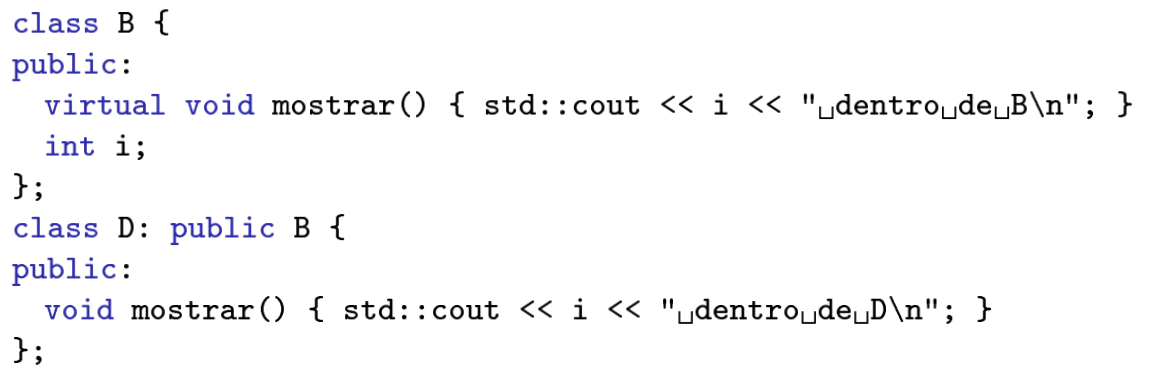
\includegraphics[width=\textwidth]{Imagenes/pol1.png}
	\end{center}
\end{figure}
La clase B es una clase \textbf{polimorfica} ya que tiene un método definido como \texttt virtual}.

La clase D tendrá dos miembros → el atributo \texttt{int i} y el método \texttt{mostrar()} , ya que hemos definido el método `\texttt{mostrar()} ) de la clase B como virtual, es decir el compilador sabe que ese método es polimórfico y por tanto se redefinirla en la clase derivada.

Esto sucede siempre y cuando la clase derivada tendrá un método con el mismo nombre y ese se defina como `virtual` en la clase base.
\begin{figure}[h]
	\begin{center}
		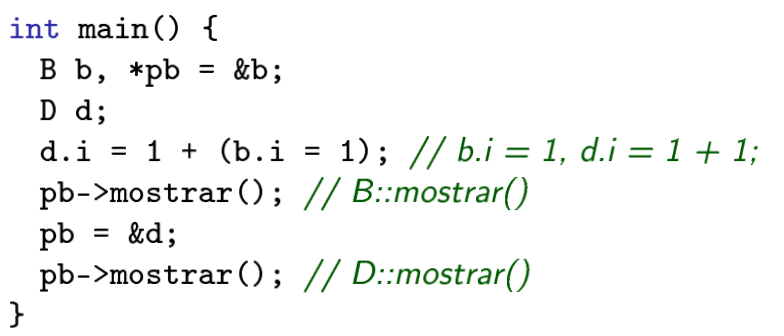
\includegraphics[width=\textwidth]{Imagenes/pol2.png}
	\end{center}
\end{figure}

En el caso de \texttt{pb ->mostrar()} ya no nos fijamos en el tipo del puntero, si no en el tipo del objeto, en este caso B. 

En \texttt{pb = &d} y \texttt{pb->mostrar()} accederá al método mostrar de la clase D, ya que el objeto al que apunta es de tipo D.

Todo esto sucede ya que hemos declarado como virtual el método mostrar, si no fuera así se llamaría siempre al método que concuerde con el tipo del puntero, en este caso el de la clase B.

\subsubsection{Ejemplo 1}

\begin{figure}[h]
	\begin{minipage}[t]{0.5\textwidth}
		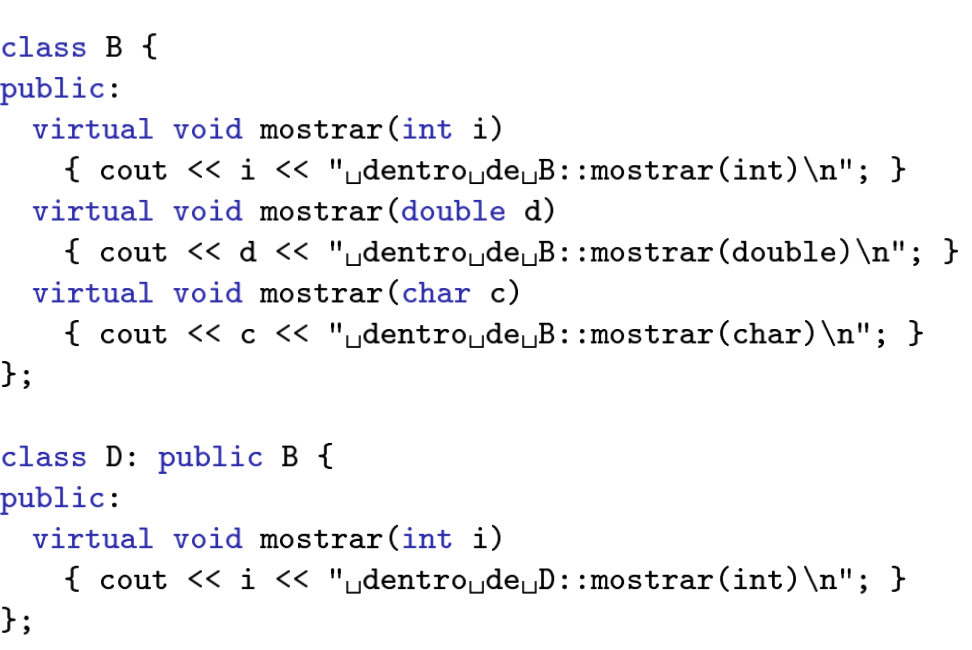
\includegraphics[width=\textwidth]{Imagenes/pol3.png}
		\caption{Cabeceras}
	\end{minipage}
	\hfill
	\begin{minipage}[t]{0.5\textwidth}
		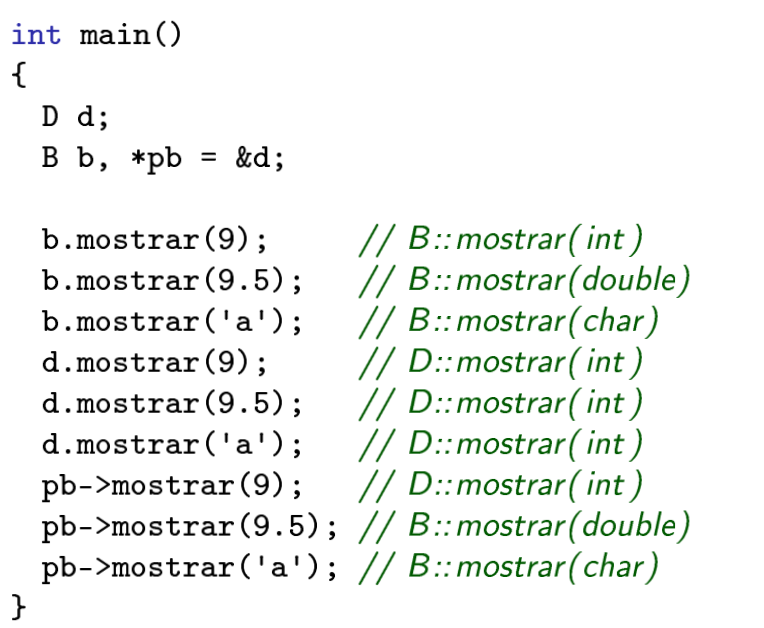
\includegraphics[width=\textwidth]{Imagenes/pol4.png}
		\caption{Código de prueba}
	\end{minipage}
\end{figure}

En este ejemplo, la clase D tiene 3 métodos dos heredados por la clase B (los que recibe un double y char) respectivamente y uno que ha sido redefinido (el que recibe un int).

Como los métodos mostrar que reciben que reciben parámetros \texttt{double}  y \texttt{char} solamente se pueden acceder a ellos cuando lo llamamos mediante un objeto de la clase B.

Si hacemos \texttt{d.mostrar('a');} nos mostrará \texttt{D::mostrar(int)}, pero si hacemos \texttt{b.mostrar(’a’);} nos mostrará \texttt{B::mostrar(char);} 

Si lo hacemos mediante punteros, se realiza un enlace dinámico que hace que comprueba el tipo del objeto de la clase, dependiendo de ese tipo llamará a un método mostrar.

Vemos que \texttt{pb} apunta a un objeto de la clase D, pero a la hora de pasarle los parámetros comprueba que método de ese objeto se corresponde a la lista de parámetros, por tanto, si se le pasa un entero y este apunta a un objeto de la clase D, se usará el método mostrar de la clase derivada D, pero como este no tiene un método redefinido para \textit{double} o \textit{char}, se llamará al método mostrar correspondiente del tipo del puntero, es decir, de la clase base B.

\subsubsection{Ejemplo 2 sin interfaz}

\begin{center}
	\begin{lstlisting}[frame=single]
class Figura{
  public:
	virtual ~Figura() {};
	virtual double area()const {return 0.0;}// por omision 
};
class Rectangulo: public Figura {
  public:
    Rectangulo(double lado_1, double lado_2);
    double area() const override;
  protected:
    double lado_1, lado_2;
};
class Circulo final: public Figura {
  public:
    Circulo(double radio);
    double area() const override;
  private:
    double radio;
};		
	\end{lstlisting}
\end{center}

Como vemos, la clase Figura es una clase polimorfica, de donde se derivan varias clases (Rectágunlo y Círculo).

El método \texttt{area()} es un método polimorfico que tendrá un comportamiento diferente en cada una de las clases derivadas.

\begin{center}
	\begin{quote}
	\textbf{Si hacemos el destructor virtual nos aseguramos que se llame al destructor de la clase derivada.\\\\
		Siempre que tengamos una clase polimorfica, su destructor debe de ser \texttt{virtual}.}

\end{quote}
\end{center}

\subsubsection{Ejemplo 2 con interfaz}
\begin{figure}[h]
	\begin{center}
		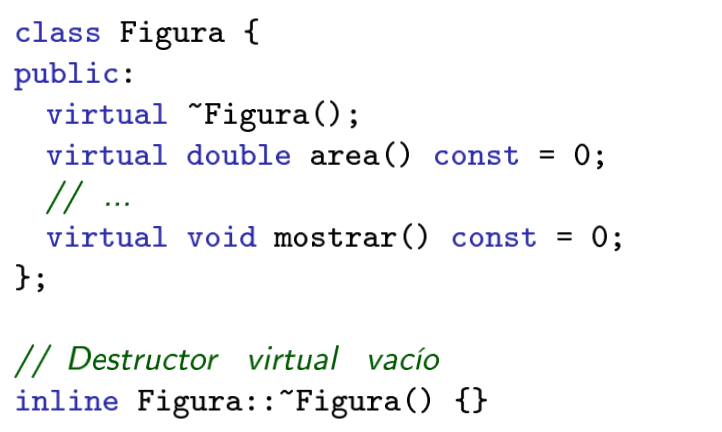
\includegraphics[width=\textwidth]{Imagenes/poli5.png}
		\caption{Definición clase Figura}
	\end{center}
\end{figure}


Convertimos la clase Figura como una clase \textbf{abstracta} haciendo que sus métodos sean \textit{virtuales puros}.

Es decir, sus métodos solo se declaran no se implementan y además no se pueden instanciar (no se pueden crear objetos de la misma), es una clase \textit{incompleta}.

\begin{figure}[h]
	\begin{minipage}{0.5\textwidth}
		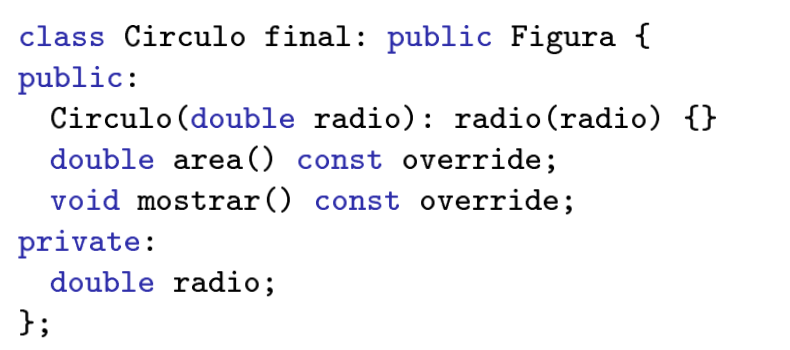
\includegraphics[width=\textwidth]{Imagenes/poli6.png}
	\end{minipage}
	\hfill
	\begin{minipage}{0.5\textwidth}
		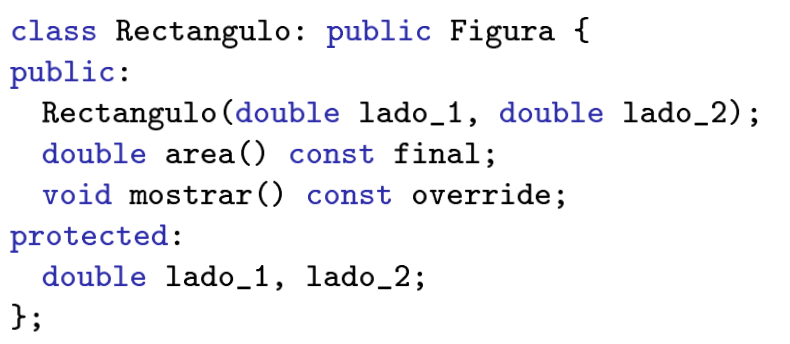
\includegraphics[width=\textwidth]{Imagenes/poli7.png}
	\end{minipage}
\end{figure}

Encontramos la \textit{keyword} \texttt{override} que le indicamos al compilador que dicho método se va a volver a implementar.

La \textit{keyword} \texttt{final} indicamos que es la versión final de la implementación de dicho método.
\newpage

\begin{figure}[h]
	\begin{center}
		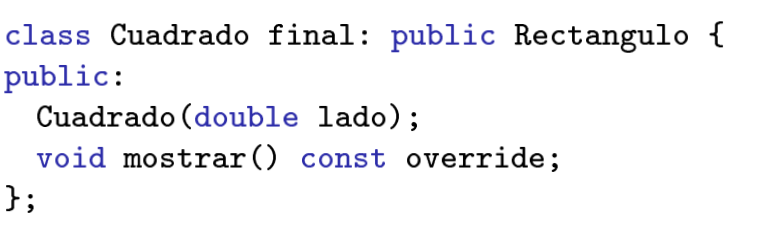
\includegraphics[width=\textwidth]{Imagenes/poli8.png}
	\end{center}
\end{figure}

Vemos que Cuadrado es una especialización de Rectángulo pero este no redefine el método \texttt{area()} debido a que se calculan igual, por eso anteriormente la definimos como final.











